\documentclass{standalone}
\usepackage[T1]{fontenc}
\usepackage[utf8]{inputenc}
\usepackage{pgf,tikz}
\usepackage{pgfplots}
\pgfplotsset{compat=1.13}

\begin{document}
\begin{tikzpicture}
  \begin{scope}
    \node[anchor=south west,inner sep=0] (image2) at (0,0) {\includegraphics[width=0.2\textwidth]{humusoftcard-small.png}};
    \begin{scope}[x={(image2.south east)},y={(image2.north west)}]
        \node[green,circle, ultra thick, inner sep=0, draw] (hground) at (0.55,0.80) {};
        \node[red,circle, ultra thick, inner sep=0, draw] (hin) at (0.85,0.80) {};
        \node[blue,circle, ultra thick, inner sep=0, draw] (hout) at (0.82,0.48) {};
%\draw[help lines,xstep=.1,ystep=.1] (0,0) grid (1,1);
%\foreach \x in {0,3,...,9} { \node [anchor=north] at (\x/10,0) {0.\x}; }
%\foreach \y in {0,3,...,9} { \node [anchor=east] at (0,\y/10) {0.\y}; }
    \end{scope}
  \end{scope}

  \begin{scope}[xshift=2.5cm, yshift=0]
    \node[anchor=south west,inner sep=0] (image) at (0,0) {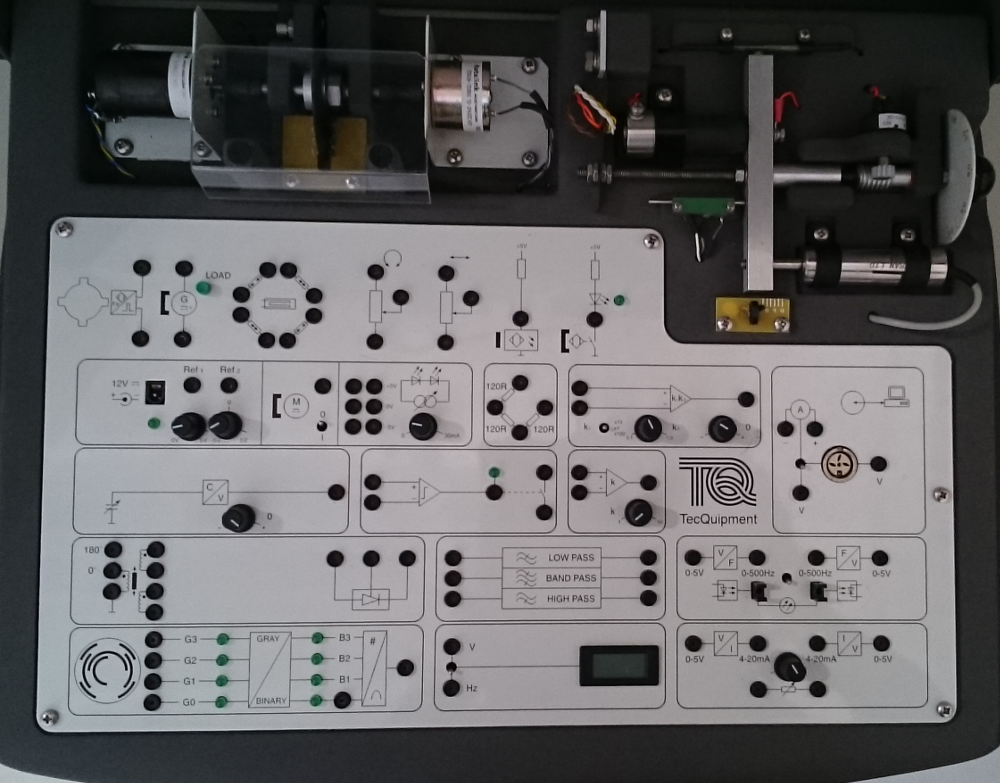
\includegraphics[width=0.5\textwidth]{TecQbox.png}};
    \begin{scope}[x={(image.south east)},y={(image.north west)}]
        \node[green,circle, ultra thick, inner sep=0, draw] (tground) at (0.185,0.565) {};
        \node[red,circle, ultra thick, inner sep=0, draw] (tach) at (0.405,0.15) {};
        \node[red,circle, ultra thick, inner sep=0, draw] (lpin) at (0.45,0.29) {};
        \node[red,circle, ultra thick, inner sep=0, draw] (lpout) at (0.65,0.29) {};
        \node[blue,circle, ultra thick, inner sep=0, draw] (motor) at (0.32,0.505) {};
%\draw[help lines,xstep=.1,ystep=.1] (0,0) grid (1,1);
%\foreach \x in {0,1,...,9} { \node [anchor=north] at (\x/10,0) {0.\x}; }
%\foreach \y in {0,1,...,9} { \node [anchor=east] at (0,\y/10) {0.\y}; }
    \end{scope}
  \end{scope}

  \draw[out=90, in=180, green, thick] (hground) to (tground);
  \draw[out=90, in=180, red, thick] (tach) to (lpin);
  \draw[out=-90, in=90, red, thick] (lpout) to (hin);
  \draw[out=40, in=-80, blue, thick] (hout) to (motor);

\end{tikzpicture}
\end{document}
